%% -------------------------------------------------------------------------
%% ------ nuweb macros (redefine as desired, or omit with "nuweb -p") ------
%% -------------------------------------------------------------------------
%\providecommand{\NWtxtMacroDefBy}{Macro defined by}
%\providecommand{\NWtxtMacroRefIn}{Macro referenced in}
%\providecommand{\NWtxtMacroNoRef}{Macro never referenced}
%\providecommand{\NWtxtDefBy}{Defined by}
%\providecommand{\NWtxtRefIn}{Referenced in}
%\providecommand{\NWtxtNoRef}{Not referenced}
%\providecommand{\NWtxtFileDefBy}{File defined by}
%\providecommand{\NWsep}{${\diamond}$}
%\providecommand{\NWlink}[2]{\hyperlink{#1}{#2}}
%\providecommand{\NWtarget}[2]{% move baseline up by \baselineskip 
%  \raisebox{\baselineskip}[1.5ex][0ex]{%
%    \mbox{%
%      \hypertarget{#1}{%
%        \raisebox{-1\baselineskip}[0ex][0ex]{%
%          \mbox{#2}%
%}}}}}
%% -------------------------------------------------------------------------
%
%
%\documentclass[11pt,oneside]{article}	%use"amsart"insteadof"article"forAMSLaTeXformat
%\usepackage{geometry}		%Seegeometry.pdftolearnthelayoutoptions.Therearelots.
%\geometry{letterpaper}		%...ora4paperora5paperor...
%%\geometry{landscape}		%Activateforforrotatedpagegeometry
%%\usepackage[parfill]{parskip}		%Activatetobeginparagraphswithanemptylineratherthananindent
%\usepackage{graphicx}				%Usepdf,png,jpg,orepsßwithpdflatex;useepsinDVImode
%								%TeXwillautomaticallyconverteps-->pdfinpdflatex		
%\usepackage{amssymb,amsmath,amsthm}
%\newtheorem{definition}{Definition}
%\usepackage[colorlinks=true]{hyperref}
%
%%----macros begin-----------------------------------------------------------------------------------
\usepackage{graphicx}
\usepackage{color}
\usepackage{amsthm}

%\renewenvironment{Shaded}{\pause\begin{snugshade}}{\end{snugshade}}
\def\twocolumns#1#2{\begin{columns}
\begin{column}{0.5\linewidth}#1\end{column}
\begin{column}{0.5\linewidth}#2\end{column}
\end{columns}}
\def\mytwocolumns#1#2#3#4{\begin{columns}
\begin{column}{#1\linewidth}#2\end{column}
\begin{column}{#3\linewidth}#4\end{column}
\end{columns}}
\def\mythreecolumns#1#2#3#4#5#6{\begin{columns}
\begin{column}{#1\linewidth}#2\end{column}
\begin{column}{#3\linewidth}#4\end{column}
\begin{column}{#5\linewidth}#6\end{column}
\end{columns}}
\def\threecolumns#1#2#3{\begin{columns}
\begin{column}{0.33\linewidth}#1\end{column}
\begin{column}{0.33\linewidth}#2\end{column}
\begin{column}{0.33\linewidth}#3\end{column}
\end{columns}}
\def\fourcolumns#1#2#3#4{\begin{columns}%
\begin{column}{0.25\linewidth}#1\end{column}%
\begin{column}{0.25\linewidth}#2\end{column}%
\begin{column}{0.25\linewidth}#3\end{column}%
\begin{column}{0.25\linewidth}#4\end{column}%
\end{columns}}

\def\conv{\mbox{\textrm{conv}\,}}
\def\aff{\mbox{\textrm{aff}\,}}
\def\E{\mathbb{E}}
\def\R{\mathbb{R}}
\def\Z{\mathbb{Z}}
\def\tex{\TeX}
\def\latex{\LaTeX}
\def\v#1{{\bf #1}}
\def\p#1{{\bf #1}}
\def\T#1{{\bf #1}}

\def\vet#1{{\left(\begin{array}{cccccccccccccccccccc}#1\end{array}\right)}}
\def\mat#1{{\left(\begin{array}{cccccccccccccccccccc}#1\end{array}\right)}}

\def\lin{\mbox{\rm lin}\,}
\def\aff{\mbox{\rm aff}\,}
\def\pos{\mbox{\rm pos}\,}
\def\cone{\mbox{\rm cone}\,}
\def\conv{\mbox{\rm conv}\,}
\newcommand{\homog}[0]{\mbox{\rm homog}\,}
\newcommand{\relint}[0]{\mbox{\rm relint}\,}

%----macros end-----------------------------------------------------------------------------------

%
\chapter{Module Lar2psm
%\footnote{This document is part of the \emph{Linear Algebraic Representation with CoChains} (LAR-CC) framework~\cite{cclar-proj:2013:00}. \today}
}
%\author{Alberto Paoluzzi}
%%\date{}							%Activatetodisplayagivendateornodate
%
%\begin{document}
%\maketitle
%%\nonstopmode

\begin{abstract}
This software module contains all the functions needed to interface the LAR data structure and/or the geometric  objects defined by it with the Plasm environment. In particular, it will include the interfaces towards the visualization primitives provided by the language.
\end{abstract}



%\tableofcontents
%\newpage

\section{Introduction}
The standard definition of vectors and matrices in plasm is the list of vector coordinates and the list of matrix rows, respectively.

\section{Implementation}

Since the present \texttt{lar2psm} module is an interface between the \texttt{larcc} library and the PLaSM language, and its various incarnations, it should allow to import the language itself (in Python, the \texttt{pyplasm} module). 
%------------------------------------------------------------------
\begin{flushleft} \small
\begin{minipage}{\linewidth} \label{scrap1}
\protect\makebox[0ex][r]{\NWtarget{nuweb2a}{\rule{0ex}{0ex}}\hspace{1em}}$\langle\,$Import the pyplasm module\nobreak\ {\footnotesize 2a}$\,\rangle\equiv$
\vspace{-1ex}
\begin{list}{}{} \item
\mbox{}\verb@from pyplasm import * @\\
\mbox{}\verb@@{\NWsep}
\end{list}
\vspace{-1ex}
\footnotesize\addtolength{\baselineskip}{-1ex}
\begin{list}{}{\setlength{\itemsep}{-\parsep}\setlength{\itemindent}{-\leftmargin}}
\item {\NWtxtMacroNoRef}.
\end{list}
\end{minipage}\\[4ex]
\end{flushleft}
%------------------------------------------------------------------

An useful utility will allow for the creation of a subdirectory from a \texttt{dirpath} \emph{string}.
%------------------------------------------------------------------
\begin{flushleft} \small
\begin{minipage}{\linewidth} \label{scrap2}
\protect\makebox[0ex][r]{\NWtarget{nuweb2b}{\rule{0ex}{0ex}}\hspace{1em}}$\langle\,$Create directory from path\nobreak\ {\footnotesize 2b}$\,\rangle\equiv$
\vspace{-1ex}
\begin{list}{}{} \item
\mbox{}\verb@import os@\\
\mbox{}\verb@def createDir(dirpath):@\\
\mbox{}\verb@    if not os.path.exists(dirpath):@\\
\mbox{}\verb@        os.makedirs(dirpath)@\\
\mbox{}\verb@@{\NWsep}
\end{list}
\vspace{-1ex}
\footnotesize\addtolength{\baselineskip}{-1ex}
\begin{list}{}{\setlength{\itemsep}{-\parsep}\setlength{\itemindent}{-\leftmargin}}
\item \NWtxtMacroRefIn\ \NWlink{nuweb2c}{2c}\NWlink{nuweb6a}{, 6a}.
\end{list}
\end{minipage}\\[4ex]
\end{flushleft}
%------------------------------------------------------------------

It may be useful to define the repository(ies) for the unit tests associated to the module:
%------------------------------------------------------------------
\begin{flushleft} \small
\begin{minipage}{\linewidth} \label{scrap3}
\protect\makebox[0ex][r]{\NWtarget{nuweb2c}{\rule{0ex}{0ex}}\hspace{1em}}\verb@"test/py/lar2psm-tests.py"@\nobreak\ {\footnotesize 2c }$\equiv$
\vspace{-1ex}
\begin{list}{}{} \item
\mbox{}\verb@@\hbox{$\langle\,$Create directory from path\nobreak\ {\footnotesize \NWlink{nuweb2b}{2b}}$\,\rangle$}\verb@@\\
\mbox{}\verb@createDir('test/py/lar2psm/')@\\
\mbox{}\verb@@{\NWsep}
\end{list}
\vspace{-2ex}
\end{minipage}\\[4ex]
\end{flushleft}
%------------------------------------------------------------------


\subsection{Convex combination}
Next we define the \texttt{CCOMB} function that accepts as input a \texttt{vectors} list (i.e., a matrix) and returns \emph{the} point their convex combination.
%------------------------------------------------------------------
\begin{flushleft} \small
\begin{minipage}{\linewidth} \label{scrap4}
\protect\makebox[0ex][r]{\NWtarget{nuweb2d}{\rule{0ex}{0ex}}\hspace{1em}}$\langle\,$Compute the convex combination of a list of vectors\nobreak\ {\footnotesize 2d}$\,\rangle\equiv$
\vspace{-1ex}
\begin{list}{}{} \item
\mbox{}\verb@import scipy as sp@\\
\mbox{}\verb@from pyplasm import *@\\
\mbox{}\verb@def CCOMB(vectors):@\\
\mbox{}\verb@    return (sp.array(VECTSUM(vectors)) / float(len(vectors))).tolist()  @\\
\mbox{}\verb@@{\NWsep}
\end{list}
\vspace{-1ex}
\footnotesize\addtolength{\baselineskip}{-1ex}
\begin{list}{}{\setlength{\itemsep}{-\parsep}\setlength{\itemindent}{-\leftmargin}}
\item \NWtxtMacroRefIn\ \NWlink{nuweb5d}{5d}.
\end{list}
\end{minipage}\\[4ex]
\end{flushleft}
%------------------------------------------------------------------

\paragraph{Unit tests}
First we test \texttt{CCOMB} with some special data, then with some random vectors.
%------------------------------------------------------------------
\begin{flushleft} \small
\begin{minipage}{\linewidth} \label{scrap5}
\protect\makebox[0ex][r]{\NWtarget{nuweb3a}{\rule{0ex}{0ex}}\hspace{1em}}\verb@"test/py/lar2psm/test-ccomb.py"@\nobreak\ {\footnotesize 3a }$\equiv$
\vspace{-1ex}
\begin{list}{}{} \item
\mbox{}\verb@@\hbox{$\langle\,$Import the module\nobreak\ ({\footnotesize \NWtarget{nuweb3b}{3b}\label{scrap6}
 }\mbox{}\verb@lar2psm@ ) {\footnotesize \NWlink{nuweb5a}{5a}}$\,\rangle$}\verb@@\\
\mbox{}\verb@from lar2psm import *@\\
\mbox{}\verb@@\hbox{$\langle\,$\texttt{CCOMB} unit tests\nobreak\ {\footnotesize \NWlink{nuweb7}{7}}$\,\rangle$}\verb@@\\
\mbox{}\verb@@{\NWsep}
\end{list}
\vspace{-2ex}
\end{minipage}\\[4ex]
\end{flushleft}
%------------------------------------------------------------------

\subsection{LAR model of a cell complex}

A very important concept introduced by the LAR package is the definition of the \emph{model} of a cell complex, as a pair made by a list of vertices, given as lists of coordinates, and a topological relation.

\begin{definition}[LAR model]
A \emph{LAR model} is a pair, e.g.~a Python tuple \emph{\texttt(V, FV)}, where:
\begin{enumerate}
\item \texttt{V} is the list of vertices, given as lists of coordinates;
\item \texttt{FV} is a \emph{cell-vertex} relation, in this case the face-vertex relation, given as a list of cells, where each cell is given as a list of vertex indices.
\end{enumerate}
\end{definition}

\paragraph{Examples} 
Some very simple examples of 0D, 1D, and 2D models follows. They are displayed in Figure~\ref{fig:lar2psm-01}.
%------------------------------------------------------------------
\begin{flushleft} \small
\begin{minipage}{\linewidth} \label{scrap7}
\protect\makebox[0ex][r]{\NWtarget{nuweb3c}{\rule{0ex}{0ex}}\hspace{1em}}$\langle\,$2D model examples\nobreak\ {\footnotesize 3c}$\,\rangle\equiv$
\vspace{-1ex}
\begin{list}{}{} \item
\mbox{}\verb@V = [[0.,0.],[1.,0.],[0.,1.],[1.,1.],[0.5,0.5]]@\\
\mbox{}\verb@VV = [[0],[1],[2],[3],[4]]@\\
\mbox{}\verb@EV = [[0,1],[0,2],[0,4],[1,3],[1,4],[2,3],[2,4],[3,4]]@\\
\mbox{}\verb@FV = [[0,1,4],[1,3,4],[2,3,4],[0,2,4]]@\\
\mbox{}\verb@@\\
\mbox{}\verb@model0d, model1d, model2d = (V,VV), (V,EV), (V,FV)@\\
\mbox{}\verb@@{\NWsep}
\end{list}
\vspace{-1ex}
\footnotesize\addtolength{\baselineskip}{-1ex}
\begin{list}{}{\setlength{\itemsep}{-\parsep}\setlength{\itemindent}{-\leftmargin}}
\item \NWtxtMacroRefIn\ \NWlink{nuweb6d}{6d}.
\end{list}
\end{minipage}\\[4ex]
\end{flushleft}
%------------------------------------------------------------------

\subsection{Function \texttt{MKPOLS}}

The function \texttt{MKPOLS} returns a list of HPC objects, i.e.~the geometric type of the PLaSM language. This list is generated to be displayed, possibly exploded, by the \texttt{pyplasm} viewer. 

Each cell \texttt{f} in the model (i.e.~each vertex list in the \texttt{FV} array of the previous example) is mapped into a polyhedral cell by the \texttt{pyplasm} operator \texttt{MKPOL}. The vertex indices are mapped from base 0 (the Python and C standard) to base 1 (the Plasm, Matlab, and FORTRAN standard).
%------------------------------------------------------------------
\begin{flushleft} \small
\begin{minipage}{\linewidth} \label{scrap8}
\protect\makebox[0ex][r]{\NWtarget{nuweb4a}{\rule{0ex}{0ex}}\hspace{1em}}$\langle\,$MaKe a list of HPC objects from a LAR model\nobreak\ {\footnotesize 4a}$\,\rangle\equiv$
\vspace{-1ex}
\begin{list}{}{} \item
\mbox{}\verb@def MKPOLS (model):@\\
\mbox{}\verb@    V, FV = model@\\
\mbox{}\verb@    pols = [MKPOL([[V[v] for v in f],[range(1,len(f)+1)], None]) for f in FV]@\\
\mbox{}\verb@    return pols  @\\
\mbox{}\verb@@{\NWsep}
\end{list}
\vspace{-1ex}
\footnotesize\addtolength{\baselineskip}{-1ex}
\begin{list}{}{\setlength{\itemsep}{-\parsep}\setlength{\itemindent}{-\leftmargin}}
\item \NWtxtMacroRefIn\ \NWlink{nuweb5d}{5d}.
\end{list}
\end{minipage}\\[4ex]
\end{flushleft}
%------------------------------------------------------------------

\paragraph{Unit tests}
Some simple 3D, 2D, 1D and 0D models are generated and visualised exploded by the file
%------------------------------------------------------------------
\begin{flushleft} \small
\begin{minipage}{\linewidth} \label{scrap9}
\protect\makebox[0ex][r]{\NWtarget{nuweb4b}{\rule{0ex}{0ex}}\hspace{1em}}\verb@"test/py/lar2psm/test-models.py"@\nobreak\ {\footnotesize 4b }$\equiv$
\vspace{-1ex}
\begin{list}{}{} \item
\mbox{}\verb@@\hbox{$\langle\,$Import the module\nobreak\ ({\footnotesize \NWtarget{nuweb4c}{4c}\label{scrap10}
 }\mbox{}\verb@lar2psm@ ) {\footnotesize \NWlink{nuweb5a}{5a}}$\,\rangle$}\verb@@\\
\mbox{}\verb@@\hbox{$\langle\,$View model examples\nobreak\ {\footnotesize \NWlink{nuweb6d}{6d}}$\,\rangle$}\verb@@\\
\mbox{}\verb@@{\NWsep}
\end{list}
\vspace{-2ex}
\end{minipage}\\[4ex]
\end{flushleft}
%------------------------------------------------------------------

\subsection{``Explosion'' of the scene}

A function \texttt{EXPLODE} used to ``explode'' an HPC scene defined as a \emph{list} of HPC values, given three real scaling parameters, \texttt{sx,sy,sz}, that are used to transform the position of the centroid of each HPC cell. HPC stands for \emph{HierarchicaL Polyhedral Complex}, the  type of plasm geometric values. Of course the assertion
\[
sx,sy,sz \geq 1.0
\]
must be true, otherways the function would induce some compenetration of the cells of the scene.

%------------------------------------------------------------------
\begin{flushleft} \small
\begin{minipage}{\linewidth} \label{scrap11}
\protect\makebox[0ex][r]{\NWtarget{nuweb4d}{\rule{0ex}{0ex}}\hspace{1em}}$\langle\,$Explode the scene using \texttt{sx,sy,sz} scaling parameters\nobreak\ {\footnotesize 4d}$\,\rangle\equiv$
\vspace{-1ex}
\begin{list}{}{} \item
\mbox{}\verb@def EXPLODE (sx,sy,sz):@\\
\mbox{}\verb@    def explode0 (scene):@\\
\mbox{}\verb@        centers = [CCOMB(S1(UKPOL(obj))) for obj in scene]@\\
\mbox{}\verb@        scalings = len(centers) * [S([1,2,3])([sx,sy,sz])]@\\
\mbox{}\verb@        scaledCenters = [UK(APPLY(pair)) for pair in@\\
\mbox{}\verb@                         zip(scalings, [MK(p) for p in centers])]@\\
\mbox{}\verb@        translVectors = [ VECTDIFF((p,q)) for (p,q) in zip(scaledCenters, centers) ]@\\
\mbox{}\verb@        translations = [ T([1,2,3])(v) for v in translVectors ]@\\
\mbox{}\verb@        return STRUCT([ t(obj) for (t,obj) in zip(translations,scene) ])@\\
\mbox{}\verb@    return explode0  @\\
\mbox{}\verb@@{\NWsep}
\end{list}
\vspace{-1ex}
\footnotesize\addtolength{\baselineskip}{-1ex}
\begin{list}{}{\setlength{\itemsep}{-\parsep}\setlength{\itemindent}{-\leftmargin}}
\item \NWtxtMacroRefIn\ \NWlink{nuweb5d}{5d}.
\end{list}
\end{minipage}\\[4ex]
\end{flushleft}
%------------------------------------------------------------------

The \texttt{EXPLODE} function is second order: it first application (to the scaling parameters) returns a partial function to be applied to the \texttt{scene}, given as a \emph{list} of HPC (Hierarchical Polyhedral Complex) objects. 
\texttt{EXPLODE} is dimension-independent, since it can be applied to points, edges, faces, 3D cells, and even to geometric values of mixed dimensionality (see Figure~\ref{fig:lar2psm-01}).

It works by computing the centroid of each object, and by applying to each of them a translation equal to the difference betwwen the scaled and the initial positions of its centroid. 
\texttt{EXPLODE}  returns a single HPC object (the assembly of input objects, properly translated)

\section{Source Output: \texttt{lar2psm} module}


\subsection{Importing a generic module}
First we define a parametric macro to allow the importing of \texttt{larcc} modules from the project repository \texttt{lib/py/}. When the user needs to import some project's module, she may call this macro as done in Section~\ref{sec:lar2psm}.
%------------------------------------------------------------------
\begin{flushleft} \small
\begin{minipage}{\linewidth} \label{scrap12}
\protect\makebox[0ex][r]{\NWtarget{nuweb5a}{\rule{0ex}{0ex}}\hspace{1em}}$\langle\,$Import the module\nobreak\ {\footnotesize 5a}$\,\rangle\equiv$
\vspace{-1ex}
\begin{list}{}{} \item
\mbox{}\verb@import sys@\\
\mbox{}\verb@sys.path.insert(0, 'lib/py/')@\\
\mbox{}\verb@import @@1\verb@@\\
\mbox{}\verb@@{\NWsep}
\end{list}
\vspace{-1ex}
\footnotesize\addtolength{\baselineskip}{-1ex}
\begin{list}{}{\setlength{\itemsep}{-\parsep}\setlength{\itemindent}{-\leftmargin}}
\item \NWtxtMacroRefIn\ \NWlink{nuweb3a}{3a}\NWlink{nuweb4b}{, 4b}\NWlink{nuweb5b}{, 5b}\NWlink{nuweb5d}{d}.
\end{list}
\end{minipage}\\[4ex]
\end{flushleft}
%------------------------------------------------------------------

\paragraph{Importing a module} A function used to import a generic \texttt{lacccc} module within the current environment is also useful.
%------------------------------------------------------------------
\begin{flushleft} \small
\begin{minipage}{\linewidth} \label{scrap13}
\protect\makebox[0ex][r]{\NWtarget{nuweb5b}{\rule{0ex}{0ex}}\hspace{1em}}$\langle\,$Function to import a generic module\nobreak\ {\footnotesize 5b}$\,\rangle\equiv$
\vspace{-1ex}
\begin{list}{}{} \item
\mbox{}\verb@def importModule(moduleName):@\\
\mbox{}\verb@   @\hbox{$\langle\,$Import the module\nobreak\ ({\footnotesize \NWtarget{nuweb5c}{5c}\label{scrap14}
 }\mbox{}\verb@moduleName@ ) {\footnotesize \NWlink{nuweb5a}{5a}}$\,\rangle$}\verb@@\\
\mbox{}\verb@@{\NWsep}
\end{list}
\vspace{-1ex}
\footnotesize\addtolength{\baselineskip}{-1ex}
\begin{list}{}{\setlength{\itemsep}{-\parsep}\setlength{\itemindent}{-\leftmargin}}
\item \NWtxtMacroRefIn\ \NWlink{nuweb5d}{5d}.
\end{list}
\end{minipage}\\[4ex]
\end{flushleft}
%------------------------------------------------------------------




\subsection{Lar2psm exporting}
\label{sec:lar2psm}
Here we assemble top-down the \texttt{lar2psm} module, by orderly listing the functional parts it is composed of. Of course, this one is the module version corresponding to the current state of the system, i.e.~to a very initial state. Other functions will be added when needed.
%------------------------------------------------------------------
\begin{flushleft} \small \label{scrap15}
\protect\makebox[0ex][r]{\NWtarget{nuweb5d}{\rule{0ex}{0ex}}\hspace{1em}}\verb@"lib/py/lar2psm.py"@\nobreak\ {\footnotesize 5d }$\equiv$
\vspace{-1ex}
\begin{list}{}{} \item
\mbox{}\verb@"""Module with functions needed to interface LAR with pyplasm"""@\\
\mbox{}\verb@@\hbox{$\langle\,$Import the module\nobreak\ ({\footnotesize \NWtarget{nuweb5e}{5e}\label{scrap16}
 }\mbox{}\verb@simplexn@ ) {\footnotesize \NWlink{nuweb5a}{5a}}$\,\rangle$}\verb@@\\
\mbox{}\verb@@\hbox{$\langle\,$Function to import a generic module\nobreak\ {\footnotesize \NWlink{nuweb5b}{5b}}$\,\rangle$}\verb@@\\
\mbox{}\verb@@\hbox{$\langle\,$Compute the convex combination of a list of vectors\nobreak\ {\footnotesize \NWlink{nuweb2d}{2d}}$\,\rangle$}\verb@@\\
\mbox{}\verb@@\hbox{$\langle\,$MaKe a list of HPC objects from a LAR model\nobreak\ {\footnotesize \NWlink{nuweb4a}{4a}}$\,\rangle$}\verb@@\\
\mbox{}\verb@@\hbox{$\langle\,$Explode the scene using \texttt{sx,sy,sz} scaling parameters\nobreak\ {\footnotesize \NWlink{nuweb4d}{4d}}$\,\rangle$}\verb@@\\
\mbox{}\verb@@{\NWsep}
\end{list}
\vspace{-2ex}
\end{flushleft}
%------------------------------------------------------------------


\section{Unit tests}

\subsection{Creation of repository of unit tests}

A possible unit test strategy is to create a directory for unit tests associated to each source file in \texttt{nuweb}. Therefore we create here a directory in \texttt{test/py/} with the same name of the present document. Of course other 

%------------------------------------------------------------------
\begin{flushleft} \small
\begin{minipage}{\linewidth} \label{scrap17}
\protect\makebox[0ex][r]{\NWtarget{nuweb6a}{\rule{0ex}{0ex}}\hspace{1em}}$\langle\,$create directory and echo of creation\nobreak\ {\footnotesize 6a}$\,\rangle\equiv$
\vspace{-1ex}
\begin{list}{}{} \item
\mbox{}\verb@@\hbox{$\langle\,$Create directory from path\nobreak\ {\footnotesize \NWlink{nuweb2b}{2b}}$\,\rangle$}\verb@@\\
\mbox{}\verb@createDir('@@1\verb@')@\\
\mbox{}\verb@print "'@@1\verb@' repository created"@\\
\mbox{}\verb@@{\NWsep}
\end{list}
\vspace{-1ex}
\footnotesize\addtolength{\baselineskip}{-1ex}
\begin{list}{}{\setlength{\itemsep}{-\parsep}\setlength{\itemindent}{-\leftmargin}}
\item {\NWtxtMacroNoRef}.
\end{list}
\end{minipage}\\[4ex]
\end{flushleft}
%------------------------------------------------------------------

%------------------------------------------------------------------
\begin{flushleft} \small
\begin{minipage}{\linewidth} \label{scrap18}
\protect\makebox[0ex][r]{\NWtarget{nuweb6b}{\rule{0ex}{0ex}}\hspace{1em}}\verb@"test/py/lar2psm/test01.py"@\nobreak\ {\footnotesize 6b }$\equiv$
\vspace{-1ex}
\begin{list}{}{} \item
\mbox{}\verb@@\hbox{$\langle\,$create directory and echo of creation:\nobreak\ ({\footnotesize \NWtarget{nuweb6c}{6c}\label{scrap19}
 }\mbox{}\verb@test/py/lar2psm/@ ) {\footnotesize ?}$\,\rangle$}\verb@@\\
\mbox{}\verb@@{\NWsep}
\end{list}
\vspace{-2ex}
\end{minipage}\\[4ex]
\end{flushleft}
%------------------------------------------------------------------


\subsection{Viewing some simplicial complexes}
Let we start producing some images, displayed in Figure~\ref{fig:lar2psm-01}, os a small simplicial complex and of its skeletons. Notice that the \texttt{+} character operates the join of lists (of HPC values).

%------------------------------------------------------------------
\begin{flushleft} \small
\begin{minipage}{\linewidth} \label{scrap20}
\protect\makebox[0ex][r]{\NWtarget{nuweb6d}{\rule{0ex}{0ex}}\hspace{1em}}$\langle\,$View model examples\nobreak\ {\footnotesize 6d}$\,\rangle\equiv$
\vspace{-1ex}
\begin{list}{}{} \item
\mbox{}\verb@from lar2psm import *@\\
\mbox{}\verb@@\hbox{$\langle\,$2D model examples\nobreak\ {\footnotesize \NWlink{nuweb3c}{3c}}$\,\rangle$}\verb@@\\
\mbox{}\verb@explode = EXPLODE(1.5,1.5,1.5)@\\
\mbox{}\verb@VIEW(explode(MKPOLS(model0d)))@\\
\mbox{}\verb@VIEW(explode(MKPOLS(model1d)))@\\
\mbox{}\verb@VIEW(explode(MKPOLS(model2d)))@\\
\mbox{}\verb@VIEW(explode(MKPOLS(model2d) + MKPOLS(model1d) + MKPOLS(model0d)))@\\
\mbox{}\verb@@{\NWsep}
\end{list}
\vspace{-1ex}
\footnotesize\addtolength{\baselineskip}{-1ex}
\begin{list}{}{\setlength{\itemsep}{-\parsep}\setlength{\itemindent}{-\leftmargin}}
\item \NWtxtMacroRefIn\ \NWlink{nuweb4b}{4b}.
\end{list}
\end{minipage}\\[4ex]
\end{flushleft}
%------------------------------------------------------------------


\begin{figure}[htbp] %  figure placement: here, top, bottom, or page
   \centering
   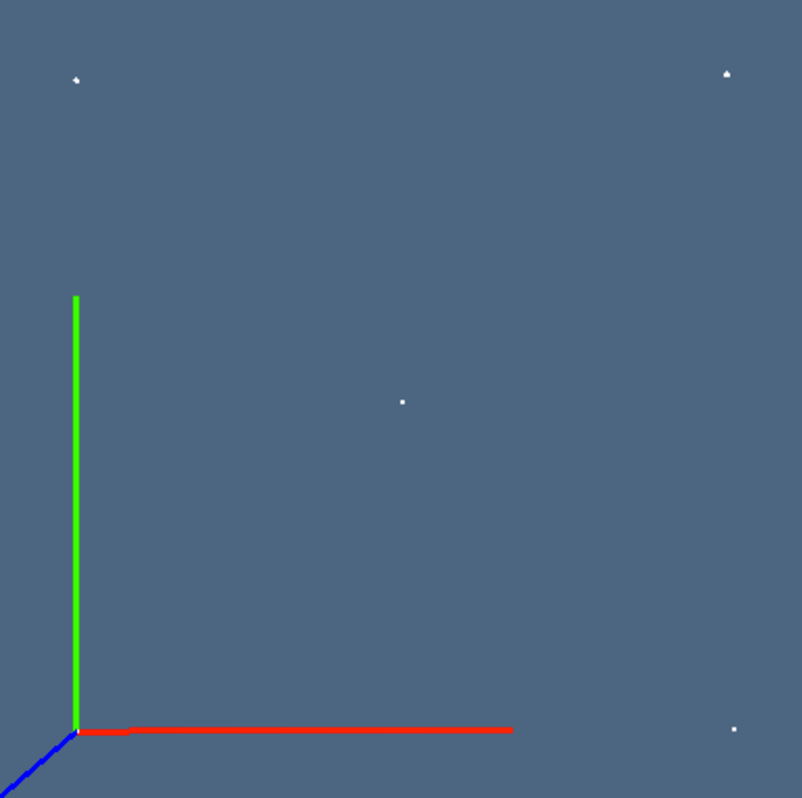
\includegraphics[height=0.245\linewidth,width=0.2425\linewidth]{images/lar2psm-01} 
   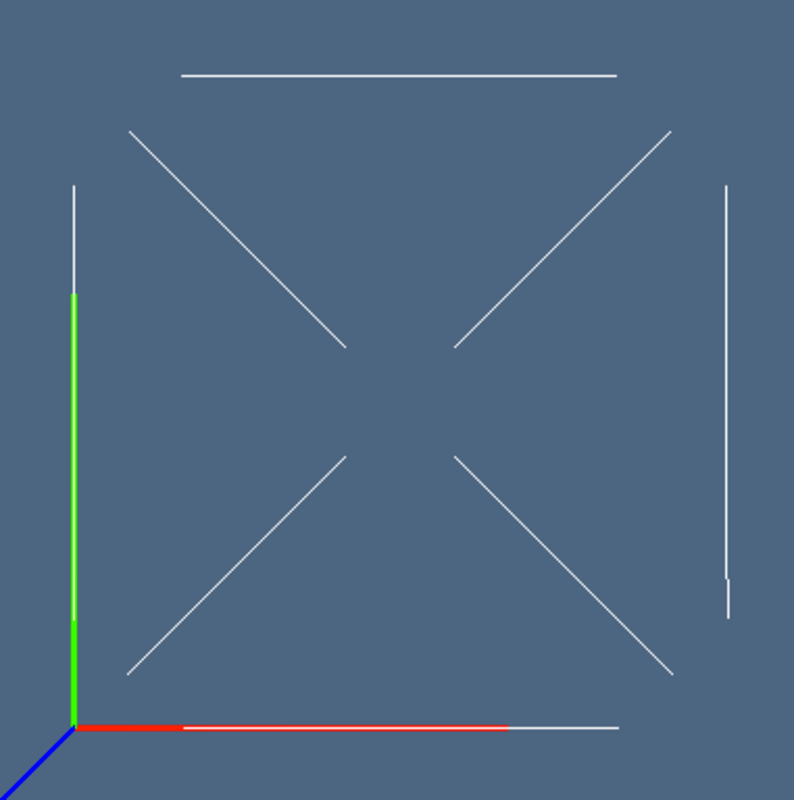
\includegraphics[height=0.245\linewidth,width=0.2425\linewidth]{images/lar2psm-02} 
   
\includegraphics[height=0.245\linewidth,width=0.2425\linewidth]{images/lar2psm-03} 
   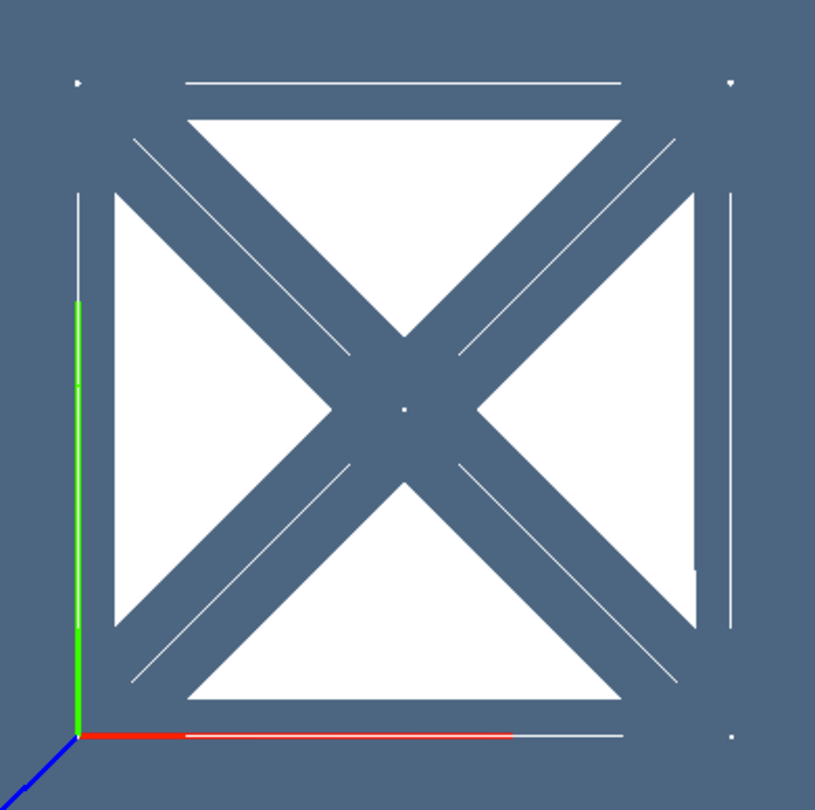
\includegraphics[height=0.245\linewidth,width=0.2425\linewidth]{images/lar2psm-04} 
   \caption{Images of the skeletons of a small simplicial complex.}
   \label{fig:lar2psm-01}
\end{figure}

\subsection{Testing convex combination of vectors}

%------------------------------------------------------------------
\begin{flushleft} \small
\begin{minipage}{\linewidth} \label{scrap21}
\protect\makebox[0ex][r]{\NWtarget{nuweb7}{\rule{0ex}{0ex}}\hspace{1em}}$\langle\,$\texttt{CCOMB} unit tests\nobreak\ {\footnotesize 7}$\,\rangle\equiv$
\vspace{-1ex}
\begin{list}{}{} \item
\mbox{}\verb@assert( CCOMB([]) == [] )@\\
\mbox{}\verb@assert( CCOMB([[0,1]]) == [0.0, 1.0] )@\\
\mbox{}\verb@assert( CCOMB([[0,1],[1,0]]) == [0.5, 0.5] )@\\
\mbox{}\verb@assert( CCOMB([[1,0,0],[0,1,0],[0,0,1]]) == [1./3,1./3,1./3])@\\
\mbox{}\verb@@\\
\mbox{}\verb@import random@\\
\mbox{}\verb@vects = [[random.random() for i in range(3)] for k in range(4)]@\\
\mbox{}\verb@assert( CCOMB([VECTSUM(vects)]) == \@\\
\mbox{}\verb@        (sp.array(CCOMB(vects)) * len(vects)).tolist() )@\\
\mbox{}\verb@@{\NWsep}
\end{list}
\vspace{-1ex}
\footnotesize\addtolength{\baselineskip}{-1ex}
\begin{list}{}{\setlength{\itemsep}{-\parsep}\setlength{\itemindent}{-\leftmargin}}
\item \NWtxtMacroRefIn\ \NWlink{nuweb3a}{3a}.
\end{list}
\end{minipage}\\[4ex]
\end{flushleft}
%------------------------------------------------------------------

\bibliographystyle{amsalpha}
\bibliography{lar2psm}

%\end{document}
